\documentclass[a4paper,11pt,pdftex, parskip]{scrreprt}
\usepackage[pdftex]{graphicx}
\usepackage[english]{babel}
\usepackage[utf8]{inputenc}
\usepackage[T1]{fontenc}
\usepackage{lmodern}
\usepackage[numbers]{natbib}
\usepackage[margin=5pt,font=small,labelfont=bf, textfont=it]{caption}
%\usepackage[reals]{layout}
\usepackage[lmargin = 2cm, rmargin = 2cm, tmargin = 2cm]{geometry}
\usepackage{listings}
\lstset{language = Python, breaklines = true}
\lstset{numbers=left, numberstyle=\small, stepnumber=2, numbersep=8pt, frame=single, aboveskip= 10pt, belowskip=10pt}


\begin{document}
%\layout*
\widowpenalty = 10000
\clubpenalty = 10000
\displaywidowpenalty = 10000

% %Abänderung Deutsch/Englisch Version False = Englisch; True = Deutsch
\newif\ifimportant
\importanttrue

\begin{titlepage}

\ifimportant
    % \title{
    %     \begin{figure}[t]
    %         \centering
    %         
\includegraphics[scale = 1, keepaspectratio]{Logos/unims.pdf}
    %         \hspace{1cm}
    %         
\includegraphics[scale = 0.9, keepaspectratio]{Logos/ifgi_logo.png}
    %     \end{figure}
    %     % \begin{figure}[t]
    %     %     \centering
    %     %     \begin{minipage}[b]{.4\linewidth}
    %     %         
\includegraphics[scale = 0.1, angle = 0]{Logos/wwu_logo.png}
    %     %        \end{minipage}
    %     %     \begin{minipage}[b]{.5\linewidth}
    %     %      
\includegraphics[scale = 0.4, angle = 0 ]{Logos/ifgi_logo.png}
    %     %     \end{minipage}
          
    %     %    \end{figure}
           
    %     \textnormal{ 
    %         \normalsize \Large 
    %        Universität Münster \\ Institut für Geoinformatik\\
    %         \vspace{3cm}
    %        % \LARGE 
    %         Proposal \\}
    %     \glqq {Automatische Erkennung von Fahrzeugen auf multi-spektralen Luftbildern mittels Deep Learning}\grqq 
    %     \vspace{1,5cm}}

   
    % \author{ 
    %     Erstgutachter: Prof. Dr. Benjamin Risse \\
    %     Zweitgutachter: Dr. Christian Knoth \\
    %     Ausgabetermin: tbd. \\
    %     \vspace{0.75cm}
    %     Abgabetermin: tbd. \\
    %     Vorgelegt von: Timo Lietmeyer \\
    %     Geboren am : 23.05.1999 \\
    %     E-Mail-Adresse: timolietmeyer@uni-muenster.de \\
    %     Matrikelnummer: 459 169 \\
    %     Studiengang: M. Sc.  Geoinformatics and Spatial Data Science
    %  }
% \else
            \title{
            \begin{figure}[t]
            \centering
            
\includegraphics[scale = 1, keepaspectratio]{Logos/unims.pdf}
            \hspace{1cm}
            
\includegraphics[scale = 0.9, keepaspectratio]{Logos/ifgi_logo.png}
            \end{figure}
            % \begin{figure}[t]
            %     \centering
            %     \begin{minipage}[b]{.4\linewidth}
            %         
\includegraphics[scale = 0.1, angle = 0]{Logos/wwu_logo.png}
            %        \end{minipage}
            %     \begin{minipage}[b]{.5\linewidth}
            % 
\includegraphics[scale = 0.4, angle = 0 ]{Logos/ifgi_logo.png}
            % \end{minipage}
            % \end{figure}
            \textnormal{ 
            \normalsize \Large 
            University of Münster \\ Institute for Geoinformatics\\
            \vspace{3cm}
            % \LARGE 
                Proposal \\}
            \glqq {Automatic detection of vehicles in multispectral aerial images using deep learning}\grqq 
            \vspace{1,5cm}}


            \author{ 
            First reviewer: Prof. Dr. Benjamin Risse \\
            Second reviewer: Dr. Christian Knoth \\
            Release date: tbd. \\
            \vspace{0.75cm}
            Deadline: tbd. \\
            Submitted by: Timo Lietmeyer \\
            Born on: 23.05.1999 \\
            E-mail address: timolietmeyer@uni-muenster.de \\
            Student ID number: 459 169 \\
            Study program: M. Sc. Geoinformatics and Spatial Data Science
            }
    \date{ }    
    
\end{titlepage}
\maketitle
%\tableofcontents

% \listoffigures \pagebreak


\setcounter{page}{1}


\ifimportant
% \section*{Motivation und Kontext}
%     Durch die leichte Verfügbarkeit von hochauflösenden Satelliten- und Luftbildern ist Detektion von Objekten weltweit möglich. Da außerdem die hohe Rechenleistung, die für maschinelles Lernen erforderlich ist, immer preiswerter wird, wird die Anwendung von künstlicher Intelligenz zur vollautomatischen Analyse immer leichter. \\
%     Das Monitoring von zerstörten (militärischen) Gerät oder Gebäudestrukturen in Konfliktregionen, wie Darfur \cite{Knoth2017} oder der Ukraine, kann durch künstliche Intelligenz unterstützt werden. Hier können Luftbiler gut genutzt werden, weil das Erstellen von Fotos vor Ort durch die Sicherheitslage am Boden in Konfliktregionen gefährlich sein kann. \\
%     Das Monitoring von militärischem Gerät an Ländergrenzen könnte benutzt werden um eine genauere Lageeinschätzung zu generieren, ob ein Konflikt bevorsteht. Es ist auch möglich die Arbeit von menschlichen Analysten unterstützen, da die Modelle Vorschläge für mögliche Detektionen und Klassifizierungen von Objekten liefern. \\
%     Maschinelles Lernen kann zur Automatisierung angewendet werden, um größere Datensätze zu verarbeiten. Eine Herausforderung hier besteht im Training der Algorithmen, da die Verfügbarkeit von Trainingsdaten limitiert ist.\\

%     Ein Anwendungszenario wäre die Auswertung des menschlichen Mobilitätsverhaltens im Rahmen des Zählen von Autos auf großen öffentlichen Parkplätzen. Hier kann auch ein Tracking von Verkehrsaufkommen durch die KI landesweit erfolgen, wenn Fahrzeuge auf einem Satellitenbild detektiert werden können. Dieser Ansatz kann genutzt werden um abzuschätzen ob mehr Parkflächen erforderlich sind oder die Anzahl der aktuellen Flächen ausreicht. Weitere Fragestellungen wären, ob es möglich ist fahrende und stehende Autos zu unterscheiden. 

%     Außerdem kann in dieser Arbeit evaluiert werden, ob die Präzision der  Objekterkennung und -klassifzierung von Fahrzeugen in elektro-optischen, multi-spektralen Luftaufnahmen durch die Nutzung von mehr Bildkanälen (NIR, IR) verbessert werden kann. Dies kann durch einen Vergleich der Ergebnisse beim Trainieren desselben Deep Learning Modells geschehen, welches jeweils nur mit 3 und einmal mit  mehr Kanälen trainiert wurde. Da Fahrzeuge relativ klein auf hochauflösenden Satellitenbildern dargestellt werden, kann auch evaluiert werden, wie gut sich ein Deep Learning Modell zur Klassifizierung sehr kleiner Objekte eignet, bzw. ob ein weiterer Kanal die Präzision verbessert.\\

%     % Es können insbesondere die Bereiche 'Objekterkennung in Satellitenaufnahmen', 'Verarbeitung und Analyse von elektro-optischen multi-spektralen Daten' sowie Deep Learning Methoden genutzt werden. Diese Deep Learning Methoden werden im Rahmen dieser Arbeit beschrieben, getestet und möglicherweise weiterentwickelt.\\
%     % Es kann ebenfalls ein Vergleich zwischen Deep Learning Modellen durchgeführt werden, die ausschließlich RGB Luftbilder als Eingabedaten nutzen und solchen, die hierfür multi-spektrale Luftbilder verwenden. Dieser Vergleich könnte im Ergebnis aufzeigen, ob und in welchem Umfang sich die Objekterkennung durch die Nutzung multi-spektraler Kanäle verbessert.

% \section*{Forschungsfragen}
% Die folgenden Forschungsfragen können im Rahmen dieser Arbeit beantwortet werden:
% \begin{itemize}
%     \item Kann man Objekterkennung und -klassifizierung auf multi-spektralen Luftbildern durch die Nutzung von vier oder mehr Kanälen verbessern?
%     \item Ist Deep Learning zur Erkennung von sehr kleinen Objekten auf hochauflösenden Luft- und/oder Satellitenbildern geeignet?
%     \item Wie hilft das IR / NIR Band dabei Objekte auf hochauflösenden Satellitenbildern zu klassifizieren und detektieren?
% \end{itemize}


% \section*{Literatur Review}
% Mit Luftbildern oder Satellitenbildern können bereits Massengräber detektiert werden \cite{Kalacska2006}. Dieser Ansatz kann in nahezu Echtzeit oder in der Vergangenheit angewendet werden \cite{Kalacska2006}. Er basiert auf Satelittenbilder, die aus verschiedene Bändern bestehen. Man kann ihn auch zur Detektion von geheimen Massengräbern nutzen \cite{Kalacska2006}. Möglicherweise ist ein Umbau zur Detektierung von Massengräbern in der Ukraine möglich \cite{Kalacska2006}. \\
% Weitere Ansätze umfassen die Erkennung von Einzelgräbern mithilfe von Air Borne Imagery \cite{Leblanc2014}. \\
% Außerdem wurden Satellitenbilder von chinesischen Krematorien genutzt, um die offiziellen Daten zur Covid Mortalität der Regierung zu überprüfen. Dies konnte in Kombination mit Augenzeugenbefragungen dafür genutzt werden, die offiziellen Zahlen zur Sterblichkeit anzuzweifeln \cite{Spiegel_article}. 

% Mit Satellitenbildern konnten bereits Zerstörungen von Hüttenstrukturen in Darfur detektiert werden \cite{Knoth2017}. Es wurden Methoden entwickelt um diese Strukturen zu erkennen und zu zählen \cite{Kemper2011}. Dies lässt sich möglicherweise auch auf Fahrzeuge anwenden \cite{Kemper2011}. \\
% Hochauflösenden Satellitenbilder können außerdem mit künstlicher Intelligenz eingesetzt werden um Armut zu analysieren \cite{Hall2023}. \\

% RGB Bilder von Drohnen können in den meisten Szenarien gut für Objekterkennung eingesetzt werden. Wärme (IR) kann die Möglichkeiten zur Objekterkennung in der Nacht oder bei verdeckten Objekten erweitern. Ein Problem ist der Mangel an verfügbaren Trainingsdaten für IR Bilder von Drohnen. Es gab Ansätze diesen Mangel mit der Erstellung von synthetischen IR Bildern zu mindern \cite{Yang2022}. \\


% %Ansätze zur Fahrzeugerkennung auf Satellitenbildern wurden bereits einer FCN Architektur basierend auf U Net zur Echtzeitanalyse erprobt. Hier wurde auch ein Trainingsdatensatz mit 80.000 Annotationen veröffentlicht, in dem jedoch kein IR Kanal vorhanden ist.  \cite{Gudius2021}

% % \begin{itemize}
% %     \item RGB Bilder von Drohnen können in den meisten Szenarien gut für Objekterkennung eingesetzt werden. Wärme (IR) kann die Möglichkeiten zur Objekterkennung in der Nacht oder bei verdeckten Objekten erweitern. Ein Problem ist der Mangel an verfügbaren Trainingsdaten für IR Bilder von Drohnen. Es gab Ansätze diesen Mangel mit der Erstellung von synthetischen IR Bildern zu mindern. \cite{Yang2022}
% %     \item Ansätze zur Fahrzeugerkennung auf Satellitenbildern wurden bereits einer FCN Architektur basierend auf U Net zur Echtzeitanalyse erprobt. Hier wurde auch ein Trainingsdatensatz mit 80.000 Annotationen veröffentlicht, in dem jedoch kein IR Kanal vorhanden ist.  \cite{Gudzius2021}
% %     \item Suchbegriffe: object detection deep learning rgb ir 
% %     \item und multispectral object detection deep learning
% %     \item KAIST multispectral Dataset
% %     \item DroneVehicle Dataset
% %     \item  AAUrainsnow Dataset
% %     \item VEDAI Dataset
% % \end{itemize}


% \section*{Methodik}
% Um Objekte auf hochauflösenden Satellitenbildern zu detektieren, bietet sich der 'You Only Look Once' (YOLO) Algorithmus an. Dieser Algorithmus, der in der Version 9 im Jahr 2024 veröffentlicht wurde, ermöglicht eine schnelle und präzise Objekterkennung. YOLO basiert auf einer einzigen neuronalen Netzwerkarchitektur, die das Bild in Raster unterteilt und für jedes Rasterfeld Vorhersagen über die Position und Klasse von Objekten trifft. 

% Die Hauptvorteile von YOLO sind seine Geschwindigkeit und Genauigkeit, die es ermöglichen, große Datensätze effizient zu analysieren. Für diese Arbeit wird YOLO verwendet, um Fahrzeuge auf Satellitenbildern zu detektieren und zu klassifizieren. Dabei könnten zusätzliche multispektrale Kanäle wie NIR oder IR integriert werden, um einen Vergleich zu dem reinen 3 Kanal RGB Training zu ermöglichen. Die Vergleichbarkeit kann gewährleistet werden, wenn die gleichen Trainings- und Testdaten verwendet werden, bei denen der einzige Unterschied das weitere Band ist.

% \subsection*{Datengrundlage}

% Das 'Vehicle Detection in Aerial Images' (VEDAI) Dataset \cite{vedai_web}  aus dem Jahr 2015 bietet sich als Datengrundlage an, da es hochauflösende Luftbilder enthält, die speziell für die Fahrzeugerkennung geeignet sind \cite{Razakarivony2015}. Es umfasst annotierte Daten, die Fahrzeuge in unterschiedlichen Szenarien, Größen und Orientierungen zeigen. Außerdem ist es ein Benchmark für die Detektion von sehr kleinen Objekten. Das Dataset enthält sowohl RGB-Bilder als auch multispektrale Daten, was es ideal für die Untersuchung der Auswirkungen zusätzlicher Kanäle wie NIR oder IR auf die Objekterkennung macht. Es sind mehr als 3700 Objekte in über 1200 Bildern annotiert. Diese Objekte sind in 8 Klassen (Boat, Camping Car, Car, Pickup Plane, Tractor, Truck, Van und Others) unterteilt und der Hintergrund der Objekte ist abwechslungsreich, was die Robustheit des trainierten Modelles erhöht. \\
% Die Auflösung der Bilder liegt bei 12.5 cm \texttimes 12.5 cm pro Pixel, was ausreichend ist um einzelne Fahrzeuge zu erkennen. Möglicherweise ist eine Downskalierung auf 30cm pro Pixel sinnvoll, um die Auflösung von Satellitenbildern zu imitieren.
 

% Die Datenaufbereitung umfasst Schritte wie das Unterteilen der Bilder in Trainings- und Testdaten, sowie die Aufbereitung der Annotationen für den YOLO Algorithmus. Nach diesen Schritten kann das Training auf dem High-Performance-Cluster (HPC) PALMA der Uni Münster erfolgen. Anhand der Ergebnismatrix wird dann ein Vergleich der beiden Modelle erfolgen, da der einzige Unterschied das weitere Band ist. 

% \section*{Erwartete Ergebnisse}

% Im Rahmen der Arbeit soll evaluiert werden, ob das Hinzufügen eines weiteren Bildkanals (wie NIR oder IR) die Präzision und Vorhersagequalität des Deep Learning Modells YOLOv9 verbessert. Es ist möglich, dass durch das Hinzufügen des Bildkanals die Genauigkeit geringer wird oder steigt, weil das Hinzufügen von Informationen die Vorhersagequalität beeinflusst. \\
% Zusammenfassend kann das Ziel dieser Arbeit eine Einschätzung sein, ob Deep Learning auf mehrkanaligen Luft- oder Satellitenbildern durch das Hinzufügen von mehr Informationen verbessert werden kann. 

 

% % \begin{itemize}
% %     \item Daten von Open Source Programm von Maxar (für erste Implementierung von Fahrzeugdetektion auf Parkplätzen mit GEOBIA?)
% %     \item (Daten aus Ahrtal / Maxar open Data Service?)
% %     \item Vielleicht ArcGIS oder QGIS Plugin am Ende rausmachen? zur einfacheren Anwendung für den normalen User?
% %     \item vielleicht Maxar Open Data Daten nutzen -> mit GEOBIA detektierte Objekte rauschneiden (mit kleinem Umgebungsrand) -> YOLO nutzen um geschnitten Objekte zu klassifizieren 
% % \end{itemize}

% % \section*{Working Plan}
% % \begin{figure}[h]
% %     \centering
% %     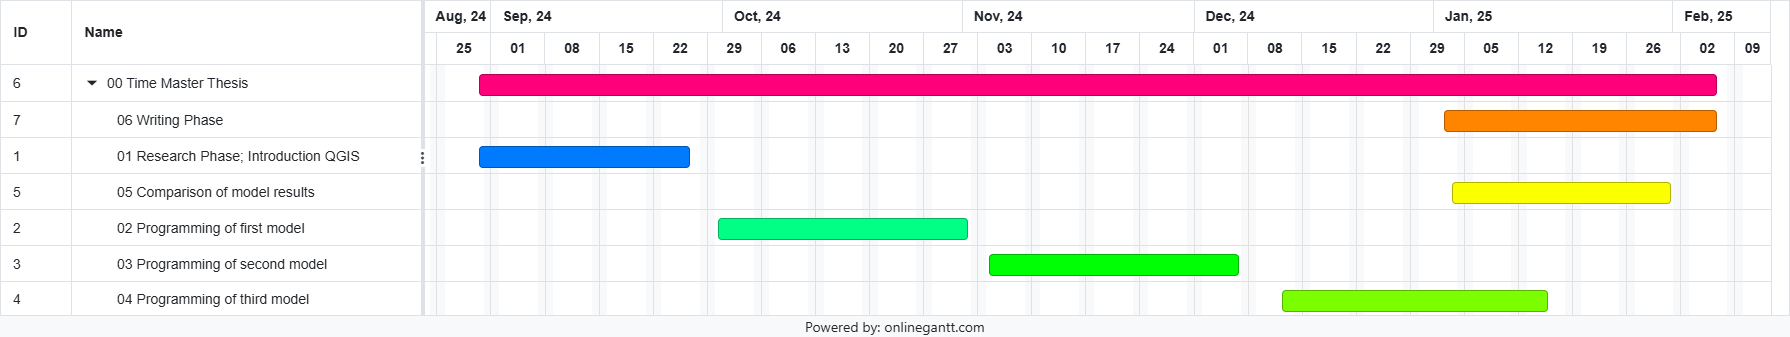
\includegraphics[scale = 0.25, keepaspectratio]{images/gantchart_ext.png}
% %     \caption{Gantt Chart for Working Plan}
% %     \label{fig:gantchart}
% % \end{figure}
% % Die Anmeldung der Masterthesis ist für den 01.09.2025 geplant und im Gantt Chart an oberster Stelle in rot dargestellt. Diese Phase soll insgesamt 117 Tage, bzw. 6 Monate vom 30.08.24-10.02.2025, dauern. \\
% % Am Anfang wird eine Literaturrecherche zur Einarbeitung in das Thema stattfinden. Diese umfasst auch die Beschäftigung mit der möglicherweise genutzten Software wie Quantum GIS (QGIS). Diese Phase dauert ca. 20 Tage, vom 30.08.-26.09.24, und ist in blau dargestellt. \\
% % Für die Entwicklung der Modelle werden jeweils 25 Tage, bzw. 3 Wochen veranschlagt. Alle drei Modelle werden hintereinander entwickelt und sind im Gantt Chart in Grüntönen dargestellt. Die Phase dauert vom 30.09-01.11.24 für das erste Modell, welches die RGB Daten zur Fahrzeugerkennung verwendet. Das zweite Modell wird direkt im Anschluss vom 04.11.2024 bis 06.12.2024 entwickelt und beinhaltet die Fahrzeugdetektion mit multi-spektralen Daten unter Benutzung des Near Infrared Bandes. Vom 12.12.2024-15.01.2025 wird das dritte Modell implementiert, welche das Infrarot Band mit Multi Spektralen Daten nutzt um Fahrzeuge zu detektieren. Bei der Entwicklungszeit von allen drei Modellen sind ein paar Tage als Puffer Zeit eingeplant. Die Entwicklung kann grob in folgende Abschnitte für jedes Modell aufgeteilt werden:
% % \begin{enumerate}
% %     \item Datenerhebung
% %     \item Datenaufbereitung
% %     \item Datensplittung in Trainings- und Validierungsdaten ( $\frac{2}{3}$ zu $\frac{1}{3}$)
% %     \item Training des Modells
% %     \item Validierung der Ergebnisse
% % \end{enumerate}

% % Der letzte Punkt wird auch in der Vergleichsphase durchgeführt und ist nicht immer sinnvoll. Insgesamt wird sich die Dauer dieser kleineren Aufgaben an dem Aufwand der Entwicklung orientieren, der im Moment noch nicht abschätzbar ist.
    
% % DIe Schreibphase ist parallel mit der Entwicklung des dritten Modells geplant und dauert 29 Tage vom 02.01.2025 bis zum 06.02.2025. Diese Phase ist in orange dargestellt. Parallel zur Schreibphase wird der Vergleich der Ergebnisse der Modell durchgeführt und direkt in die Masterthesis eingearbeitet. Diese Phase dauert vom 03.01.2025-31.01.2025 und ist in Gelb dargestellt. \\
% % Zum Ende der Schreibphase sind noch ein paar Tage zur Problemlösung als Puffer eingeplant.




% \fi

    \section*{Motivation and Context}
    The easy availability of high-resolution satellite and aerial images makes it possible to detect objects worldwide. Furthermore, the high computing power required for machine learning is becoming increasingly cheaper, making the application of artificial intelligence for fully automated analysis easier.
    The monitoring of destroyed (military) equipment or building structures in conflict regions, such as Darfur \cite{Knoth2017} or Ukraine, can be supported by artificial intelligence. Aerial imagery can be used well here because the security situation on the ground in conflict regions can make it dangerous to take photos on the ground. \\
    Monitoring military equipment at national borders could be used to generate a more accurate assessment of the situation to determine whether a conflict is imminent. It is also possible to support the work of human analysts, as the models provide suggestions for possible detections and classifications of objects. \\
    Machine learning can be applied to automate the process of processing larger data sets. One challenge here is training the algorithms, since the availability of training data is limited.\\

    One application scenario would be to evaluate human mobility behavior when counting cars in large public parking lots. Here, traffic volumes can also be tracked nationwide by the AI if vehicles can be detected on a satellite image. This approach can be used to estimate whether more parking spaces are needed or whether the number of current spaces is sufficient. Further questions would be whether it is possible to distinguish between moving and stationary cars. 

    Furthermore, this work can evaluate whether the precision of object detection and classification of vehicles in electro-optical, multi-spectral aerial images can be improved by using more image channels (NIR, IR). This can be done by comparing the results when training the same deep learning model with only 3 and once with more channels. Since vehicles appear relatively small on high-resolution satellite images, it is also possible to evaluate how well a deep learning model is suited to classifying very small objects, or whether an additional channel improves precision.


    \section*{Research Questions}
The following research questions can be answered in the context of this work:
\begin{itemize}
  \item Can object detection and classification on multi-spectral aerial images be improved by using four or more channels?
  \item Is deep learning suitable for detecting very small objects on high-resolution aerial and/or satellite images?
  \item How does the IR / NIR band help to classify and detect objects on high-resolution satellite images?
\end{itemize}

\section*{Literature review}
Aerial or satellite images can already be used to detect mass graves \cite{Kalacska2006}. This approach can be applied in near real-time or in the past \cite{Kalacska2006}. It is based on satellite images that consist of different bands and can also be used to detect secret mass graves \cite{Kalacska2006}. Here it could  be possible to modify it to detect mass graves in Ukraine \cite{Kalacska2006}. \\
Other approaches include the detection of individual graves using airborne imagery \cite{Leblanc2014}. \\
In addition, satellite images of Chinese crematoria were used to verify the official government data on Covid mortality. This, in combination with eyewitness interviews, was used to cast doubt on the official mortality figures \cite{Spiegel_article}. 

Satellite images have already been used to detect the destruction of hut structures in Darfur \cite{Knoth2017}. Methods have been developed to detect and count these structures \cite{Kemper2011}. This may also be possible to apply to vehicles \cite{Kemper2011}. \\
High-resolution satellite images can also be used with artificial intelligence to analyze poverty \cite{Hall2023}. \\

RGB images from drones are sufficient for object detection in most scenarios. Thermal (IR) images can extend the possibilities for object detection at night or for hidden objects. One problem is the lack of available training data for IR images from drones. There have been approaches to mitigate this problem by creating synthetic IR images \cite{Yang2022}. \\



\section*{Methods}
The 'You Only Look Once' (YOLO) algorithm is ideal for detecting objects on high-resolution satellite images. This algorithm, which was released in version 9 in 2024, enables fast and accurate object detection. YOLO is based on a single neural network architecture that divides the image into grids and makes predictions about the position and class of objects for each grid. 

The main advantages of YOLO are its speed and accuracy, which make it possible to efficiently analyze large data sets. For this work, YOLO is used to detect and classify vehicles on satellite images. Additional multispectral channels such as NIR or IR could be integrated to allow a comparison to the pure 3-channel RGB training. Comparability can be ensured if the same training and test data is used, where the only difference is the additional band.

\subsection*{Data basis}

The 'Vehicle Detection in Aerial Images' (VEDAI) dataset \cite{vedai_web} from 2015 is suitable as a data basis because it contains high-resolution aerial images that are specifically suitable for vehicle detection \cite{Razakarivony2015}. It includes annotated data showing vehicles in different scenarios, sizes and orientations. It is also a benchmark for the detection of very small objects. The dataset contains both RGB images and multispectral data, making it ideal for investigating the effects of additional channels such as NIR or IR on object detection. There are more than 3700 objects annotated in over 1200 images. These objects are grouped into 8 classes (Boat, Camping Car, Car, Pickup Plane, Tractor, Truck, Van and Others) and the background of the objects is varied, which increases the robustness of the trained model. \\
The resolution of the images is 12.5 cm \texttimes 12.5 cm per pixel, which is sufficient to recognize individual vehicles. It may be useful to downscale to 30 cm per pixel to imitate the resolution of satellite images.
 

Data preparation includes steps such as dividing the images into training and test data, as well as preparing the annotations for the YOLO algorithm. After these steps, the training can take place on the high-performance cluster (HPC) PALMA at the University of Münster. Based on the result matrix, a comparison of the two models will then be made, since the only difference is the additional band. 

\section*{Expected results}

The aim of the work is to evaluate whether adding another image channel (such as NIR or IR) improves the precision and prediction quality of the deep learning model YOLOv9. It is possible that adding the image channel will decrease or increase the accuracy because adding information affects the prediction quality. \\
In summary, the goal of this work can be an assessment of whether deep learning on multi-channel aerial or satellite images can be improved by adding more information.





\appendix

\bibliographystyle{unsrtnat}
\bibliography{Bibliography}






\end{document}



